\documentclass[11pt,a4paper,oneside,footinclude=true,headinclude=true]{scrbook}
\usepackage[algoruled, noend]{algorithm2e}
\usepackage{a4wide}
\usepackage{graphicx}
\usepackage[left=4cm]{geometry} % okraje
\usepackage{latexsym}% kvuli symbolum v grafech vkladanych z gnuplotu
\usepackage{amsfonts}
\usepackage{amssymb,amsmath}
\usepackage[cp1250]{inputenc}
\usepackage[czech,english]{babel}
\usepackage[T1]{fontenc}
\usepackage{listings}
\usepackage{subfigure}
\selectlanguage{english}
\usepackage{verbatim}
\usepackage{enumerate}
\usepackage{color}
\usepackage{float}
\usepackage{url}
\usepackage{epsfig}
\usepackage{natbib}
\usepackage{latexsym}
\usepackage{amsmath}
\usepackage{amssymb}
\usepackage{bm}
\usepackage{graphicx}
\usepackage{wrapfig}
\usepackage{fancybox}
\usepackage{setspace}
\usepackage{hyperref}

\lstset{language=C++, basicstyle=\scriptsize, commentstyle=, showstringspaces=true} 

\title{Large-scale Numerical Simulations of Magneto-Hydrodynamics Phenomena in Astrophysics} 
\author{Lukas Korous} 
\renewcommand{\sectionmark}[1]{\markright{#1}{}}

\pagenumbering{gobble}
\begin{document}

\newcommand{\lo}{\left(}
\newcommand{\ro}{\right)} 
\newcommand{\bs}[1]{\textit{\textbf{#1}}}
\newcommand{\bsm}[1]{\boldsymbol{#1}}
\newcommand{\pds}[2]{\frac{\partial{#1}}{\partial{#2}}}
\newcommand{\pdv}[2]{\frac{\partial{#1}}{\partial{\bs{#2}}}}
\renewcommand{\d}[2]{\frac{d{#1}}{d{#2}}}
\newcommand{\mc}[1]{\mathcal{#1}}
\newcommand{\phib}{\bsm{\varphi}}
\newcommand{\esssup}{\operatornamewithlimits{ess\,sup}}

% Jakub Cerveny.

\newtheorem{definition}{Definition}[chapter]
\newtheorem{remark}{Remark}[chapter]
\newtheorem{conjecture}{Conjecture}[chapter]
\newtheorem{exercise}{Exercise}[chapter]
\newtheorem{theorem}{Theorem}[chapter]
\newtheorem{lemma}{Lemma}[chapter]
\newtheorem{corollary}{Corollary}[chapter]
\newtheorem{proposition}{Proposition}[chapter]

\newenvironment{proof}[1][Proof]{\begin{trivlist}
\item[\hskip \labelsep {\bfseries #1}]}{\end{trivlist}}


\def\be{\begin{equation}}
\def\ee{\end{equation}}
\def\bfig{\begin{figure}}
\def\efig{\end{figure}}
\def\bd{\begin{displaymath}}
\def\ed{\end{displaymath}}
\def\ba{\begin{array}}
\def\ea{\end{array}}

\newcommand{\bfa}{\mbox{\boldmath $a$}}
\newcommand{\bfb}{\mbox{\boldmath $b$}}
\newcommand{\bfc}{\mbox{\boldmath $c$}}
\newcommand{\bfd}{\mbox{\boldmath $d$}}
\newcommand{\bfe}{\mbox{\boldmath $e$}}
\newcommand{\bff}{\mbox{\boldmath $f$}}
\newcommand{\bfg}{\mbox{\boldmath $g$}}
\newcommand{\bfh}{\mbox{\boldmath $h$}}
\newcommand{\bfi}{\mbox{\boldmath $i$}}
\newcommand{\bfj}{\mbox{\boldmath $j$}}
\newcommand{\bfk}{\mbox{\boldmath $k$}}
\newcommand{\bfl}{\mbox{\boldmath $l$}}
\newcommand{\bfm}{\mbox{\boldmath $m$}}
\newcommand{\bfn}{\mbox{\boldmath $n$}}
\newcommand{\bfo}{\mbox{\boldmath $o$}}
\newcommand{\bfp}{\mbox{\boldmath $p$}}
\newcommand{\bfq}{\mbox{\boldmath $q$}}
\newcommand{\bfr}{\mbox{\boldmath $r$}}
\newcommand{\bfs}{\mbox{\boldmath $s$}}
\newcommand{\bft}{\mbox{\boldmath $t$}}
\newcommand{\bfu}{\mbox{\boldmath $u$}}
\newcommand{\bfuhp}{\mbox{{\boldmath $u$}$_{h, p}$}}
\newcommand{\bfv}{\mbox{\boldmath $v$}}
\newcommand{\bfvhp}{\mbox{{\boldmath $v$}$_{h, p}$}}
\newcommand{\bfw}{\mbox{\boldmath $w$}}
\newcommand{\bfx}{\mbox{\boldmath $x$}}
\newcommand{\bfy}{\mbox{\boldmath $y$}}
\newcommand{\bfz}{\mbox{\boldmath $z$}}
%
\newcommand{\bfA}{\mbox{\boldmath $A$}}
\newcommand{\bfB}{\mbox{\boldmath $B$}}
\newcommand{\bfC}{\mbox{\boldmath $C$}}
\newcommand{\bfD}{\mbox{\boldmath $D$}}
\newcommand{\bfE}{\mbox{\boldmath $E$}}
\newcommand{\bfF}{\mbox{\boldmath $F$}}
\newcommand{\bfG}{\mbox{\boldmath $G$}}
\newcommand{\bfH}{\mbox{\boldmath $H$}}
\newcommand{\bfI}{\mbox{\boldmath $I$}}
\newcommand{\bfJ}{\mbox{\boldmath $J$}}
\newcommand{\bfK}{\mbox{\boldmath $K$}}
\newcommand{\bfL}{\mbox{\boldmath $L$}}
\newcommand{\bfM}{\mbox{\boldmath $M$}}
\newcommand{\bfN}{\mbox{\boldmath $N$}}
\newcommand{\bfO}{\mbox{\boldmath $O$}}
\newcommand{\bfP}{\mbox{\boldmath $P$}}
\newcommand{\bfQ}{\mbox{\boldmath $Q$}}
\newcommand{\bfR}{\mbox{\boldmath $R$}}
\newcommand{\bfS}{\mbox{\boldmath $S$}}
\newcommand{\bfT}{\mbox{\boldmath $T$}}
\newcommand{\bfU}{\mbox{\boldmath $U$}}
\newcommand{\bfV}{\mbox{\boldmath $V$}}
\newcommand{\bfW}{\mbox{\boldmath $W$}}
\newcommand{\bfX}{\mbox{\boldmath $X$}}
\newcommand{\bfY}{\mbox{\boldmath $Y$}}
\newcommand{\bfZ}{\mbox{\boldmath $Z$}}
\newcommand{\bfone}{\mbox{\boldmath $1$}}
%
\def\Hcurl{{\bfH({\rm curl})}}
\def\Hdiv{{\bfH({\rm div})}}
%\def\R{{\rm I\hspace{-0.9mm}R}}
\def\R{\boldmath R}
\def\C{\boldmath C}
\def\Q{\boldmath Q}

%
\def\calB{{\cal B}}
\def\calF{{\cal F}}
\def\calM{{\cal M}}
\def\calS{{\cal S}}
\def\calA{{\cal A}}
\def\calG{{\cal G}}
\def\calE{{\cal E}}
%\def\cale{{\cal e}}
\def\calL{{\cal L}}
\def\calD{{\cal D}}
\def\calI{{\cal I}}
\def\calJ{{\cal J}}
\def\calT{{\cal T}}
\def\calY{{\cal Y}}
\def\calZ{{\cal Z}}
%
\newcommand{\ds}{\displaystyle}
%
\newcommand{\bfalp}{\mbox{\boldmath $\alpha$}}
\newcommand{\bfbet}{\mbox{\boldmath $\beta$}}
\newcommand{\bfgam}{\mbox{\boldmath $\gamma$}}
\newcommand{\bfdel}{\mbox{\boldmath $\delta$}}
\newcommand{\bfeps}{\mbox{\boldmath $\epsilon$}}
\newcommand{\bfvareps}{\mbox{\boldmath $\varepsilon$}}
\newcommand{\bfzet}{\mbox{\boldmath $\zeta$}}
\newcommand{\bfeta}{\mbox{\boldmath $\eta$}}
\newcommand{\bfthet}{\mbox{\boldmath $\theta$}}
\newcommand{\bfiot}{\mbox{\boldmath $\iota$}}
\newcommand{\bfkap}{\mbox{\boldmath $\kappa$}}
\newcommand{\bflam}{\mbox{\boldmath $\lambda$}}
\newcommand{\bfmu}{\mbox{\boldmath $\mu$}}
\newcommand{\bfnu}{\mbox{\boldmath $\nu$}}
\newcommand{\bfxi}{\mbox{\boldmath $\xi$}}
\newcommand{\bfomega}{\mbox{\boldmath $\omega$}}
\newcommand{\bfzeta}{\mbox{\boldmath $\zeta$}}
\newcommand{\bfpi}{\mbox{\boldmath $\pi$}}
\newcommand{\bfrho}{\mbox{\boldmath $\rho$}}
\newcommand{\bfsig}{\mbox{\boldmath $\sigma$}}
\newcommand{\bftau}{\mbox{\boldmath $\tau$}}
\newcommand{\bfups}{\mbox{\boldmath $\upsilon$}}
\newcommand{\bfphi}{\mbox{\boldmath $\phi$}}
\newcommand{\bfvarphi}{\mbox{\boldmath $\varphi$}}
\newcommand{\bfchi}{\mbox{\boldmath $\chi$}}
\newcommand{\bfpsi}{\mbox{\boldmath $\psi$}}
\newcommand{\bfome}{\mbox{\boldmath $\omega$}}
%
\newcommand{\bfGam}{\mbox{\boldmath $\Gamma$}}
\newcommand{\bfDel}{\mbox{\boldmath $\Delta$}}
\newcommand{\bfThet}{\mbox{\boldmath $\Theta$}}
\newcommand{\bfLam}{\mbox{\boldmath $\Lambda$}}
\newcommand{\bfXi}{\mbox{\boldmath $\Xi$}}
\newcommand{\bfPi}{\mbox{\boldmath $\Pi$}}
\newcommand{\bfSig}{\mbox{\boldmath $\Sigma$}}
\newcommand{\bfUps}{\mbox{\boldmath $\Upsilon$}}
\newcommand{\bfPhi}{\mbox{\boldmath $\Phi$}}
\newcommand{\bfPsi}{\mbox{\boldmath $\Psi$}}
\newcommand{\bfOme}{\mbox{\boldmath $\Omega$}}

\newcommand{\ptl}{{\partial}}
\newcommand{\nab}{{\nabla}}

\newcommand{\Tau}{{\cal{T}}}

\def \span {{\rm span}}

\newcommand\dS{\mbox{d\boldmath$S$}}
\renewcommand\O{{\cal O}}
\renewcommand\P{{\cal P}}
\renewcommand\H{{\cal H}}

\newcommand{\bfptl}{\mbox{\boldmath $\partial$}}
\newcommand{\bfell}{\mbox{\boldmath $\ell$}}
\newcommand{\bfnab}{\mbox{\boldmath $\nabla$}}
\newcommand{\bfinfty}{\mbox{\boldmath $\infty$}}
\newcommand{\bfto}{\mbox{\boldmath $\to$}}
\newcommand{\doubleIR}{\mbox{$I \!\!\!\! R$}}
\newcommand{\doubleIC}{\mbox{$I \!\!\! C$}}
\newcommand{\dlbracket}{\mbox{$[ \! |$}}
\newcommand{\drbracket}{\mbox{$] \! |$}}
\newcommand{\dlx}{\mbox{$x \!\!\!\! x$}}
\newcommand{\notO}{\mbox{$O \!\!\!\! /$}}
\newcommand{\tm}{\mbox{$^{TM}$}}

\newcommand{\dd}{\mathrm d}
\newcommand{\der}[2]{\frac{{\dd} #1}{{\dd} #2}}
\newcommand{\pard}[2]{\frac{\partial #1}{\partial #2}}
\newcommand{\pardx}[3]{\frac{\partial^{#1} #2}{\partial #3^{#1}}}
\newcommand{\vct}[1]{\boldsymbol{#1}}
\newcommand{\op}[1]{{\cal{#1}}}
\newcommand{\lp}{\left(}
\newcommand{\rp}{\right)}
\newcommand{\lb}{\left[}
\newcommand{\rb}{\right]}
\newcommand{\lsp}{\left\langle}
\newcommand{\rsp}{\right\rangle}
\newcommand{\lcb}{\left\lbrace}
\newcommand{\rcb}{\right\rbrace}
\newcommand{\li}{\left.}
\newcommand{\ri}{\right.}
\newcommand{\tens}[1]{\mbox{\boldmath$#1$}}

\newcommand{\mrH}{\mathrm{H}}
\newcommand{\mrF}{\mathrm{F}}
\newcommand{\mrv}{\mathrm{v}}
\newcommand{\mrvh}{\mathrm{v}}
\newcommand{\mrw}{\mathrm{w}}
\newcommand{\mrPsi}{\mathrm{\Psi}}

\begin{titlepage}
    \begin{center}
        
        \vspace*{3em}
        \textsc{\LARGE University of West Bohemia in Pilsen}\\[0.5em]
        \textsc{\LARGE Faculty of Electrotechnics}\\[5em]
        
        {\Large Doctoral thesis}\vspace*{1em}
        \rule{\linewidth}{0.5mm}
        \\[1em]
        {\huge \textsc{Large-scale Numerical Simulations of Magneto-Hydrodynamics Phenomena in Astrophysics} \\[0.4cm]}
        \rule{\linewidth}{0.5mm}
        \\[3em]
        
        {\Large Mgr. Luk� \textsc{Korous}}
        \vfill
        {\large 2016}
    \end{center}
\end{titlepage}

\normalsize
\setcounter{page}{1}
\tableofcontents

\newpage

\noindent
....................česky..................
\vspace{10mm}

\noindent
Title: Large-scale Numerical Simulations of Magneto-Hydrodynamics Phenomena in Astrophysics\\
Author: Lukáš Korous\\
Department: .........................\\
Supervisor: .........................\\
Supervisor's e-mail address: .........................\\

\noindent Abstract:
The objective of this Doctoral Thesis was to develop, implement and test new algorithms for the large-scale solution of nonstationary compressible MHD equations based on higher-order discontinuous Galerkin (DG) methods. The basis for the new methods will be the discontinuous Galerkin methods and adaptive mesh refinement (AMR) algorithms. The new algorithms will be implemented and tested in the framework of the open source library Deal.II, and they will be applied to selected problems of MHD in astrophysics, namely the magnetic reconnection phenomena. \\

\noindent Keywords: numerical simulation, finite element method, MHD equations, adaptivity, discontinuous Galerkin method, astrophysics, solar flares, CME, magnetic reconnection

\newpage



\tableofcontents

\section{Notation}
In the entire work, we use the notation specified in \ref{table:notation} on page \pageref{table:notation}.

\begin{table}
    \centering
    \begin{tabular}{ |c|l| } 
        \hline
        Symbol & Meaning \\ 
        \hline
        $a$ & a scalar quantity "a"\\
        $\bfa$ & a 3-element vector "a"\\
        $a_i$ & the i-th component of a vector $\bfa$ \\
        $\mrA$ & an 8-element vector "A" \\
        \hline
        $\rho$ & Density \\ 
        $\bfpi$ & Momentum \\ 
        $\mu$ & Permeability \\ 
        $\mu_0$ & Permeability of vacuum\\ 
        $t$ & Time variable\\ 
        $\bfx$ & Space variable \\ 
        $p$ & Pressure \\ 
        $\bfu$ & Velocity \\ 
        $u$ & Magnitude of velocity, i.e. $|\bfu|$ \\ 
        $\bfB$ & Magnetic flux density \\ 
        $\bfJ$ & Current density\\ 
        $B$ & Magnitude of magnetic flux density, i.e. $|\bfB|$ \\ 
        $\bfE$ & Electric field\\ 
        $e$ & Internal energy density \\ 
        $c$ & Speed of light\\ 
        $\bfg$ & Gravitational acceleration\\ 
        $\sigma$ & Conductivity, $\sigma = \frac{1}{\eta}$\\ 
        $\eta$ & Electrical restisistivity, $\eta = \frac{1}{\sigma}$\\
        $c_v$ & Specific heat at constant volume\\
        $c_p$ & Specific heat at constant pressure\\
        $\gamma$ & Poisson adiabatic constant\\
        $\theta$ & Absolute temperature\\
        $\bfq$ & Heat flux\\
        $q$ & Electric charge\\
        $\bff$ & Density of force acting on fluid\\
        $\bfF_L$ & Lorentz force, $\bfF_L = q\lo\bfE + \bfu\times\bfB\ro$\\
        $\bff_L$ & Lorentz force density, $\bff_L = \rho_q\bfE + \bfJ\times\bfB$\\
        $\varepsilon$ & Electrical permittivity\\
        $\varepsilon_0$ & Electrical permittivity of vacuum\\
        $\rho_q$ & Charge density\\
        $U_k$ & Kinetic energy, $U_k = \rho\frac{u^2}{2}$ \\ 
        $U_m$ & Magnetic energy, $U_m = \frac{B^2}{2{}\mu_0}$ \\ 
        $U$ & Total energy, $U = U_k + U_m + \rho e$ \\ 
        $\tilde{U}$ & Hydrodynamic energy, $\tilde{U} = U - U_m$ \\ 
        $\bfn$ & Unit outer normal \\ 
        \hline
    \end{tabular}
    \caption{Notation}
    \label{table:notation}
\end{table}



\chapter{Introduction}
\pagenumbering{arabic}
\setcounter{page}{1}

The term magnetohydrodynamics (MHD) covers all physical phenomena that involve both electromagnetic (EM) field and a fluid that carries the EM field. Such phenomena are very interesting, yet very complex to study. The behavior of such a fluid is utilized in some industrial applications - liquid-metal cooling of nuclear reactors, magnetic fluid in dampers, sensors for precise measuring of angular velocities, etc. Such phenomena occur in nature as well - the most significant of which are definitely the processes that take place inside and on the surface of stars - which is the topic of the next section.

\subsection{Magnetohydrodynamics in Astrophysics}
There are several phenomena in the universe that we can look at as Magneto-hydro-dynamic in nature - planets consisting of metals, interplanetary space, but mainly - stars. If we talk about the nearest star - and the only one we are able to study well enough - the Sun - these phenomena include those that occur in the sun's photosphere (the layer of sun that is visible): sun spots, but also phenomena that occur 'above' the sun: in sun's chromosphere, or even corona (solar flares) - even phenomena that originate from the Sun, but then spread through our solar system - solar winds, space weather. All these phenomena have a large impact on the lives of all of us. For example solar flares (that are often followed by ejection of mass out of the Sun - the so called coronal mass ejections - CMEs) have impact on the Earth's magnetic field which in turn has impact on the electronic communication down on Earth (because the communication satellites used for transmissions may be damaged by the disturbances in the magnetic field). Also people operating at high altitudes, both in airplanes and manned space missions are exposed to the energetic particles coming from the Sun (this term is sometimes called \textit{cosmic rays}). For all the above reasons, it is of great importance to understand the phenomena of space weather, and other MHD phenomena that occur in space.
\subsubsection{Magnetic reconnection}

Magnetic reconnection occurs within electrically charged gases called plasmas. These charged particles interact strongly with magnetic fields, but at the same time their motions modify the magnetic field. Plasmas behave unlike what we regularly experience on Earth because they travel with their own set of magnetic fields entrapped in the material. Changing magnetic fields affect the way charged particles move and vice versa, so the net effect is a complex, constantly-adjusting system that is sensitive to minute variations.

Under normal conditions, the magnetic field lines inside plasmas don't break or merge with other field lines. But sometimes, as field lines get close to each other, the entire pattern changes and everything realign into a new configuration. The amount of energy released can be formidable. Magnetic reconnection taps into the stored energy of the magnetic field, converting it into heat and kinetic energy that sends particles streaming out along the field lines.

Solar flares, which are among the phenomena which are the most important to study, are driven by magnetic reconnection - and thus studying magnetic reconnection is of utmost importance.

\section{State of the art}
Only recently, the scientific computation community, due to the advances in computer and supercomputer capabilities, has started with non-trivial numerical simulations of such complex physical phenomena that the MHD model describes. Since both for industrial applications, and obviously for astrophysical application of the MHD model, it is quite expensive (or downright impossible) to perform any experiments, the benefit of being able to simulate the phenomena on a computer is very large.\\
There exist several available numerical simulation codes, such as \citep{athena}, \citep{zeus}, \citep{ramses}, \citep{honzaFD}. These codes have been successfully applied to a range of problems in astrophysics.\\
There are many numerical methods implemented in these codes, such as the finite difference method (\citep{honzaFD}), finite volume method (\citep{ramses}), and the (continous) finite element method (\citep{honzaFem}).

There have been some attempts to employ also the discontinuous Galerkin method (\citep{mhdDg}, \citep{mhdDg2}), but so far no open-source generic software employing this method is available.

The reason for the development of a new code is two-fold. First, there is a unique collaboration between the Astronomical Institute of the Czech Academy of Sciences and the University of West Bohemia, where astrophysicists work together with electrical engineers (from theoretical and numerical modeling backgrounds), and the developed code will be usable for both simulating of astrophysical MHD phenomena, and industrial MHD applications.
\paragraph{}
Second, the newly developed code is based on locally-adaptive Discontinuous Galerkin method, which yields several advantages over the existing codes (which use e.g. finite difference, or finite volumes methods) developed at institutions of such high quality as \emph{Princeton} - \citep{athena}, \citep{zeus}. The advantages are especially of performance, and automation nature - method of higher order together with local mesh refinement yields results qualitatively and quantitatively comparable to low order uniform mesh methods, but with computational cost that can easily be an order of magnitude smaller. Automation is mentioned here related to the AMR, automatic mesh refinement, which, without user interaction, can optimize the computational triangulation for a particular time instance in the evolution of the modeled phenomena.
\paragraph{}
Another benefit (namely over \citep{zeus})of the newly created software are the use of modern object-oriented programming techniques and experience gained on creating finite element software (\citep{ja1}, \citep{ja2}, \citep{ja3}).
The implementation related to this work is written in the C++ language, with the use of existing software packages that are proven, and used by a wide community of researchers all over the world - deal.II (\citep{deal}), UMFPACK (\citep{umfpack}), Paraview(\url{http://www.paraview.org/}).

\paragraph{}
The state of the art of numerical simulation of magnetohydrodynamics can be summarized as a state when the mathematical theory of the equations is quite solid, but the methods to solve the equations numerically in the most optimal and fast way are still being improved. The numerical solution is not merely about theoretical convergence rates and attributes of the particular method, but also the actual implementation plays an important role - i.e. programming, hardware, and software, and execution, both before, during, and very importantly after the actual method invocation (of the so-called \textit{postprocessing} of results). In all aspects of implementation, there is space for new approaches, new ideas, new milestones, that can expand the capabilities of today's numerical solution of magnetohydrodynamics phenomena.

\chapter{Mathematical model}
In this chapter, the mathematical model will be derived from basic equations, its weak formulation will be presented, and the complete mathematical problem which is solved will be described.
\section{Derivation of the mathematical model}

\subsection{Initial setup}

We consider a time interval $\left(0,T\right)$ and space domain $\Omega_{t}\subset \mathbb{R}^3$ occupied by a fluid at time $t$.
By $\mathcal{M}$ we denote the space-time domain in consideration: 
\begin{equation}\label{M}
\mathcal{M}=\left\{\left(\textbf{\textit{x}},t\right);\\\textbf{\textit{x}}\in\Omega_{t},t\in\left(0,T\right)\right \}.
\end{equation}
Moreover we assume that $\mathcal{M}$ is an open set.

\subsubsection{Assumptions}
When dealing with MHD phenomena in plasma, the following rules apply
\begin{itemize}
    \item We assume that the fluid is inviscid.
    \item We assume that the fluid is compressible.
    \item We consider only the so-called \textit{perfect gas} or \textit{ideal gas} whose state variables satisfy the following \textit{equation of state}
    \begin{equation}\label{start_therm}
    p = R\theta\rho,
    \end{equation}
    where $\rho$ denotes density, $\theta$ denotes the absolute temperature, and $R$ is the \textit{gas constant}, which is defined as 
    \begin{equation}
    R = c_p - c_v.
    \end{equation}
    In the above, $c_p, c_v$ are specific heat at constant pressure, and at constant volume.
\end{itemize}

\subsection{Euler's equations of compressible flow}
This system of equation reads

\begin{eqnarray}
\label{ContinuityEq} \pds{\rho}{t} + \nabla\cdot\left(\bfpi\right) & = & 0\\
\label{NSEq} \pds{\bfpi}{t} + \nabla\cdot\left(\bfpi\otimes\bfu\right)& = & \rho\bff - \nabla\,p,\\
\label{EnergyEq} \pds{\tilde{U}}{t} + \nabla\cdot\lo{\tilde{U}}\bfu\ro & = & \rho\bff\cdot\bfu \,-\,\nabla\cdot\lo{p}\bfu\ro + \nabla\cdot\bfq,
\end{eqnarray}
where $\bfpi$ is momentum, $p$ pressure, $U$ total energy. Moreover, $\bfu$ denotes velocity, $\bff$ density of the force acting on the fluid, and $\bfq$ is the heat flux. By $\otimes$, we denote the \textit{tensor product}:
\begin{displaymath}
\bs{a}\otimes\bs{b} =
\left(
\begin{array}{ccc}
a_1b_1 & a_1b_2 & a_1b_3 \\
a_2b_1 & a_2b_2 & a_2b_3 \\
a_3b_1 & a_3b_2 & a_3b_3
\end{array}
\right).
\end{displaymath}

Moreover, the following relations hold:
\begin{eqnarray}
\tilde{U} & = & \rho e + U_k,\\
p & = & \lo{}\gamma-1\ro\lo{\tilde{U}}-U_k\ro, \label{therm_1}\\
\theta & = & \lo{\tilde{U}}/{\rho}-\left|\bfu\right|^2/2\ro/{c_v}.
\end{eqnarray}

This system is simply called the \textit{compressible Euler equations} for a heat-conductive perfect gas. The individual equations are called the \textit{continuity equation}(\ref{ContinuityEq}), the \textit{Navier-Stokes equations} (\ref{NSEq}), and the \textit{energy equation} (\ref{EnergyEq}).

For the force density $f$ we assume that only the Lorentz force and gravity act upon the fluid:
$$
\label{ForceEq} \bff = \bff_L + \bfg.
$$


\subsection{Maxwell's equations of electromagnetism}
In this work, we use Maxwell's equations with the assumption of constant electrical permittivity, and constant permeability. This system of equation reads
\begin{eqnarray}
\label{Ampere} \nabla \times \bfB & = & \mu_0 \lo \bfJ + \varepsilon_0 \pds{\bfE}{t}\ro\\\
\label{Faraday} \nabla \times \bfE & = & -\pds{\bfB}{t}\\
\label{Gauss} \nabla \cdot \bfE & = & \frac{\rho_q}{\varepsilon_0}\\
\label{GaussMag} \nabla \cdot \bfB & = &0,
\end{eqnarray}
where $\bfB$ denotes magnetic flux density, $\bfE$ denotes electric field, $\bfJ$ denotes current density, $\varepsilon_0$ is permittivity of vacuum, and $\rho_q$ is electric charge density.
The individual equations are known as Faraday's law(\ref{Faraday}), Ampere's law(\ref{Ampere}), and Gauss's laws(\ref{Gauss}, \ref{GaussMag}).


\subsection{Derived relations between electromagnetic quantities}
Further relations that are useful when deriving the MHD equations are:
\begin{eqnarray}
\label{U_mEq} \frac{\text{d}}{\text{d}t} U_m & = & \frac{1}{\mu_0}\nabla \cdot \lo \bfB\times\bfE\ro - \bfE\cdot\bfJ,\\
\label{Ohm} \bfE & = & -u \times \bfB + \frac{\eta}{\mu_0}\bfJ,\\
\label{InductionEq} \pds{\bfB}{t} + \nabla \times \lo \bfB \times \bfu \ro & = & -\frac{1}{\mu_0} \nabla \times \lo \eta \nabla \times \bfB \ro,
\end{eqnarray}
where $\mu_0$ denotes permeability of vacuum, $\eta$ is resistivity, and $U_m$ is magnetic energy.
The equation \ref{Ohm} is the differential form of the \textit{Ohm's law}, the equation \ref{InductionEq} is the \textit{induction equation}.

Applying now \ref{ForceEq} to \ref{NSEq}, \ref{EnergyEq}, we obtain:
\begin{eqnarray}
\label{NSEq1} \pds{\bfpi}{t} + \nabla\cdot\left(\bfpi\otimes\bfu\right)& = & \rho_q\bfE + \bfJ\times\bfB + \rho\bfg - \nabla\,p,\\
\label{EnergyEq1} \pds{\tilde{U}}{t} + \nabla\cdot\lo{\tilde{U}}\bfu\ro & = & \rho_q\bfE\cdot\bfu + \bfJ\times\bfB\cdot\bfu + \rho\bfg\cdot\bfu \,-\,\nabla\cdot\lo{p}\bfu\ro + \nabla\cdot\bfq.
\end{eqnarray}
The adjusted energy equation \ref{EnergyEq1} does not include the magnetic energy $U_m$, which we do want to include in the MHD equations. To achieve this, we employ \ref{U_mEq} - \ref{InductionEq} and rearrange and we obtain the final energy equation
\be
\label{EnergyEqPrefinal} \pds{U}{t} = -\nabla\cdot\left[\bfpi\lo \frac{u^2}{2} + e\ro + p \bfu - \frac{1}{\mu_0}\bfB\times\bfE\right] + \rho \bfg \cdot \bfu + \nabla\cdot\bfq.
\ee

\subsection{Simplifying assumptions}
In what follows, we will make several simplifying assumptions, according to which we will get a system of equations that will adequately respect the physical model, yet will be easier to be solved.
\subsubsection{Negligible time derivative of electric field}
For the time increments that we are concerned with, the time derivative in \ref{Ampere} (the so-called \textit{Maxwell's displacement current})is
very small. To estimate the minimum time increment value $\tau$ which would allow us to neglect the derivative, take the ratio of the two terms on the right hand side of \ref{Ampere}:
\begin{equation}
\varepsilon_0 \frac{\pds{\bfE}{t}}{\bfJ} \approx \frac{\frac{\varepsilon_0 \bfE}{\tau}}{\sigma\bfE} \approx \frac{\varepsilon_0}{\sigma \tau} \approx \frac{10^{-11}}{\tau}.
\end{equation}
This means for time scales much greater than $10^{-11}$ seconds, the time derivative of $\bfE$ can be neglected. As a consequence Equation \ref{Ampere} can be written as:
\begin{equation}
\label{Assumption1} \nabla \times \bfB = \mu_0 \bfJ.
\end{equation}
Using \ref{Assumption1}, we can write
\begin{equation}
\label{Asssumption11} \mu_0 \bfJ \times \bfB = \lo\bfB\cdot\nabla\ro\bfB - \nabla\frac{B^2}{2} = \nabla\cdot\lo\bfB\bfB\ro - \nabla\frac{B^2}{2},
\end{equation}
where the last equality comes from \ref{GaussMag}. And using \ref{Asssumption11} we can rewrite \ref{NSEq1} as
\be
\label{NSEq2} \pds{\bfpi}{t} + \nabla\cdot\left(\bfpi\otimes\bfu\right) =  q\bfE + \nabla\cdot\lo\frac{1}{\mu_0}\bfB\bfB - \frac{B^2}{2}\mathrm{I}\ro + \rho\bfg - \nabla\,p
\ee

\subsubsection{Negligible electric field in the Navier-Stokes equations}
The magnitude of electric field is smaller than the magnetic field by the factor $\frac{u^2}{c^2}$, so we can neglect the term $\rho_q\bfE$ on the right-hand-side of \ref{NSEq2}.

\subsubsection{Negligible heat fluxes}
Since the heat transfer accounts for a negligible contribution to the overall energy transfer, we neglect the heat flux terms, i.e. we set $\bfq = \mathbf{0}$ in the energy equation \ref{EnergyEqPrefinal}.

\subsection{Adding the induction equation}
The induction equation \ref{InductionEq} can be rearranged in the following way:
\begin{eqnarray}
\pds{\bfB}{t} + \nabla \times \lo \bfB \times \bfu \ro & = & -\frac{1}{\mu_0} \nabla \times \lo \eta \nabla \times \bfB \ro\\
\label{InductionPreFinal} \pds{\bfB}{t} & = & - \nabla \times \lo \bfu \otimes \bfB - \bfB \otimes \bfu \ro + \frac{1}{\mu_{0}\sigma} \lo \nabla^2 \bfB \ro.
\end{eqnarray}
Now we can form the system of MHD equations:
\begin{eqnarray}
\label{ContinuityEqFinal} \pds{\rho}{t} & = & - \nabla\cdot\left(\bfpi\right),\\
\label{NSEqFinal} \pds{\bfpi}{t} & = & - \nabla\cdot\left(\bfpi\otimes\bfu\right) + \nabla\cdot\lo\frac{1}{\mu_0}\bfB\bfB - \frac{B^2}{2}\mathrm{I}\ro + \rho\bfg - \nabla\,p,\\
\label{EnergyEqFinal} \pds{U}{t} & = & -\nabla\cdot\left[\bfpi\lo \frac{u^2}{2} + e\ro + p \bfu - \frac{1}{\mu_0}\bfB\times\bfE\right] + \rho \bfg \cdot \bfu\\
\label{InductionFinal} \pds{\bfB}{t} & = & - \nabla \times \lo \bfu \otimes \bfB - \bfB \otimes \bfu \ro + \frac{1}{\mu_{0}\sigma} \lo \nabla^2 \bfB \ro.
\end{eqnarray}
This form suggests that rewriting these equations into a more suitable (for numerical calculations) conservative form shall be possible.
\subsection{Conservative form of the MHD equations}
A conservative form of a system of equations takes the form of
\be
\label{conservativeGeneric} \pds{\mrPsi}{t} + \nabla \cdot \mrF\lo\mrPsi\ro = \mrS,
\ee
where $\mrPsi$ is the so-called \textit{state vector}, $\mrF_i,\ i = 1, 2, 3$ are the so-called \textit{fluxes}, and $\mrS$ is the so-called \textit{source term}.
\paragraph{}
Rewriting the system of equations \ref{ContinuityEqFinal} - \ref{InductionFinal} to the form \ref{conservativeGeneric} is fairly straightforward.
We obtain the following:
\begin{eqnarray}
\mrPsi & = & \lo\begin{array}{c}\rho \\ \pi_1 \\ \pi_2 \\ \pi_3 \\ U \\ B_1 \\ B_2 \\ B_3 \\ \end{array}\ro,\\\mrF_i & = & \lo\begin{array}{c} \pi_i \\ \frac{\pi_1 \pi_i}{\rho} - B_1 B_i + \frac12 \delta_{1i} \lo p + U_m\ro \\ \frac{\pi_2 \pi_i}{\rho} - B_1 B_i + \frac12 \delta_{2i} \lo p + U_m\ro \\ \frac{\pi_3 \pi_i}{\rho} - B_1 B_i + \frac12 \delta_{3i} \lo p + U_m\ro \\ \frac{\pi_i}{\rho} \lo \frac{\gamma}{\gamma - 1} p + U_k\ro + 2\eta\varepsilon_{ijk} J_j B_k + \frac{2}{\rho} \varepsilon_{ijk} \lo \pi_k B_i - \pi_i B_k\ro B_k  \\ \frac{\pi_i B_1 - \pi_1 B_i}{\rho} + \eta \varepsilon_{1ij} J_j \\ \frac{\pi_i B_2 - \pi_2 B_i}{\rho} + \eta \varepsilon_{2ij} J_j \\ \frac{\pi_i B_3 - \pi_3 B_i}{\rho} + \eta \varepsilon_{3ij} J_j \\ \end{array}\ro,\\
\mrS & = & \lo\begin{array}{c}0 \\ \rho g_1 \\ \rho g_2 \\ \rho g_3 \\ \bfpi \cdot \bfg \\ 0 \\ 0 \\ 0 \\ \end{array}\ro,
\end{eqnarray}
where $J_j = \lo\nabla\times\bfB\ro_j$.
\subsection{Solution considerations}
For mathematical clarity, we should state, that the solution to the equations \ref{conservativeGeneric} is such a function
\be
\label{HardSln} \mrPsi\in C^1\lo\lo0, T\ro, \left[C^1\lo\Omega_{t}\ro\right]^8\ro;\ \mrPsii\in C^1\lo\lo0, T\ro, C^2\lo\Omega_{t}\ro\ro,\,i = 6, 7, 8,
\ee
for which \ref{conservativeGeneric} holds for all $\bfx\in\Omega_t,\ t\in\lo 0, T\ro$. The kind of spaces we used in the definition is called a Bochner space.
\paragraph{}
Because such a requirement on the solution $\mrPsi$ is rather strong, we shall instead look for a so-called \textit{weak solution}, which is specified in the coming sections.

\input{math-model-weak-form}

\section{Weak formulation of the problem}
The DG method is defined by first considering the weak formulation of the equations \ref{conservativeGeneric} obtained by multiplying the equations at every time instance $t$ by a (vector-valued) test function $\mrv\in W_t$, where $W_t$ is a suitable space of (vector-valued) functions $W_t = \lo W_1, ..., W_8\ro$, integrating over the space domain $\Omega_{t}$, and performing integration by parts.
We start with multiplying \ref{conservativeGeneric} by a test function:
\be
\pds{\mrPsi}{t} \mrv + \lo\nabla \cdot \mrF\lo\mrPsi\ro\ro \mrv = \mrS \mrv,
\ee
then we integrate over $\Omega_{t}$:
\be
\int_{\Omega_{t}} \pds{\mrPsi}{t} \mrv + \int_{\Omega_{t}} \lo\nabla \cdot \mrF\lo\mrPsi\ro\ro \mrv = \int_{\Omega_{t}} \mrS \mrv,
\ee
and finally we integrate by parts:
\be
\label{WeakFinal} \int_{\Omega_{t}} \pds{\mrPsi}{t} \mrv - \int_{\Omega_{t}}\mrF\lo\mrPsi\ro \lo\nabla \cdot \mrv\ro + \int_{\partial\Omega_{t}} \lo\mrF\lo\mrPsi\ro \cdot \bfn \ro\mrv = \int_{\Omega_{t}} \mrS \mrv,
\ee
where the terms $\mrF\lo\mrPsi\ro \lo\nabla \cdot \mrv\ro; \lo\mrF\lo\mrPsi\ro \cdot \bfn \ro\mrv$ are meant as a component-wise multiplication.
\paragraph{}
Now without going into detail, we can conclude, that a suitable space $W$ would be
\be
\label{Sobolev} W_t = \left[H^{1}\lo\Omega_t\ro\right]^8,
\ee
and we shall look for a solution to the \ref{WeakFinal} in the same space $W_t$ at every time instance $t$. We shall not relax the requirement for continuity of time-derivatives we imposed for the \textit{hard solution} \ref{HardSln} for reasons discussed later, and we arrive at the following Bochner space in which we are looking for a weak solution of \ref{conservativeGeneric}:
\be
\label{Bochner} W = C^{1}\lo\lo0, T\ro, W_t\ro.
\ee

To sum up we can define the \textit{weak solution $\mrPsi = \mrPsi\lo(t, \bfx\ro)$} of MHD equations \ref{conservativeGeneric} as
\begin{enumerate}
    \label{weakSlnDef}
    \item $\mrPsi\lo(t, \bfx\ro) \in W$ defined in \ref{Bochner}
    \item \ref{WeakFinal} holds for all $t\in\lo0, T\ro$, and all $\mrv\in W_t$.
    \item $\mrPsi\lo0, \bfx\ro = \Pi \mrPsi^0\lo\bfx\ro$,
\end{enumerate}
where $\Pi$ is a projection of the initial condition $\mrPsi^0$ onto $W_0$.

\section{Boundary conditions}
\label{section:bcs}

\subsection{Essential (inflow) boundary conditions}

Since the solution \ref{weakSlnDef} of the problem specified in \ref{WeakFinal} is not influenced by its values on the boundary $\Omega_t$, we are not able to employ standard essential boundary conditions of the form $u\left(x, y, z\right) = u_D\left(x, y, z\right)$ with a known $u_D$.
If such a condition is required from the physical nature of the described phenomenon (as often is the case), it is only implied by the use of fluxes - as one can see in the last integrand $\mathrm{F}\lo\mathrm{\Psi}\ro \mathrm{v}$ in \ref{WeakFinal}.


\subsection{Outflow (do-nothing) boundary conditions}
If we want to model free boundary, that is not in any way present as an actual physical boundary or interface, this is usually achieved by specifying the fluxes through the boundary $\mathrm{F}\lo\mathrm{\Psi}\ro \mathrm{v}$ in \ref{WeakFinal} to be zero:
$$
\mathrm{F}\lo\mathrm{\Psi}\lo\bfx\ro\ro = 0\ \forall\bfx\in\partial\Omega_t\, \forall t\in \lo0, T\ro.
$$


\subsection{Periodic boundary conditions}
Periodic boundary condition is always specified on two parts $\Gamma_1, \Gamma_2$ of the domain boundary that share the bijection mapping between points:
$$
\left[x_1, y_1, z_1\right] \leftrightarrow \left[x_2, y_2, z_2\right] \forall \left[x_1, y_1, z_1\right] \in \Gamma_1,\ \forall \left[x_2, y_2, z_2\right] \in \Gamma_2,
$$
so that for each pair of related points $\left[x_1, y_1, z_1\right] \leftrightarrow \left[x_2, y_2, z_2\right]$, the values must be the same:
$$
u\left(\left[x_1, y_1, z_1\right]\right) = u\left(\left[x_2, y_2, z_2\right]\right) \forall \left[x_1, y_1, z_1\right] \in \Gamma_1,\ \forall \left[x_2, y_2, z_2\right] \in \Gamma_2:\, \left[x_1, y_1, z_1\right] \leftrightarrow \left[x_2, y_2, z_2\right].
$$


\chapter{Numerical model}
The weak formulation of the problem we obtained in \ref{weakSlnDef} still posses a problematic attribute - the space defined in \ref{Bochner} is of infinite dimension, and therefore we would need to employ analytical methods to find the solution \ref{weakSlnDef} in such a space. The equation \ref{WeakFinal} is however rather impossible to be solved analytically, and we have to utilize some sort of numerical simulation - which in turn needs to operate on finite-dimensional spaces. But we need to make sure that the simplifying (reducing) assumptions we make on the way to the numerical model are acceptable so that the numerical solution we obtain converges (as we reduce the discretization size) to the solution defined in \ref{weakSlnDef}.

\paragraph{}
In this chapter we shall consider that $\Omega_t = \Omega\, \forall t \in \lo 0, T\ro $, i.e. the computational domain does not change with respect to time. There are approaches to numerical simulation of MHD phenomena without this condition in place, which utilize the exact same general approach described in this work plus they add additional steps in the algorithm. These are outside of the scope of this work. Also, we always take $\Omega \subset \mathbb{R}^3$.

\section{Triangulation}
\label{section:triangulation}
We start with leaving the time-derivative untouched, and focus on the discretization in space for now - we are performing a \textit{space semidiscretization}.
\paragraph{}
First step in the process of the discretization is to divide the computational domain $\overline{\Omega}$ into a finite number of subsets with properties described below. These subsets form the set, further denoted by $ T_h$, called the \textit{triangulation of the domain $\Omega$}. The parameter $h>0$ of the triangulation usually represents maximum of diameters of all elements $K\in T_h$. The elements $K\in T_h$ are in the context of the finite volume method called $finite\ volumes$.
\\\ \\Properties of $ T_h$:
\begin{enumerate}
    \item Each $K\in T_h$ is closed and connected with its interior $K^{\circ}\neq\emptyset$.
    \item Each $K\in T_h$ has a Lipschitz boundary.
    \item$\cup_{K\in T_h}K\,=\,\overline{\Omega}$
    \item If $K_1,K_2\in T_h$, $K_1\neq{K_2}$, then $K_1^{\circ}\cap{T}_2^{\circ} = \emptyset$.
\end{enumerate}
\paragraph{}
In our case of the three-dimensional problem, we assume that the domain $\Omega$ is obtained as an approximation of the original computational domain (also denoted by $\Omega$), and the triangulation is chosen accordingly to the following attributes:
\renewcommand{\labelenumi}{\Alph{enumi})}
\begin{enumerate}
    \item Each $K\in T_h$ is a closed rectangular parallelepiped, possibly with curved edges.
    \item For $K_1,K_2\in T_h,\,K_1\neq{K}_2$ we have either $K_1\cap{K}_2 = \emptyset$ or $K_1,K_2$ share one edge (if the shared edge is a whole common edge, we call the triangulation \emph{regular}), or $K_1,K_2$ share one vertex, or $K_1,K_2$ share one face.
    \item$\cup_{K\in T_h}K\,=\,\overline{\Omega}.$
\end{enumerate}
Furthermore
\be
\label{Idef}  T_h = \left\{K_i, i\in I\right\},
\ee
where $I\subset Z^+ = \left\{0, 1, 2, ...\right\}$ is a suitable index set.\\
By $\Gamma_{ij}$ we denote a common face between two
neighboring elements $K_i$ and $K_j$. We set 
$$s
\lo i\ro = \left\{j\in I; K_j \text{ is a neighbor of } K_i\right\}.
$$
The boundary $\partial\Omega$ is formed by a finite number of faces of elements $K_i$ adjecent to
$\partial\Omega$. We denote all these boundary faces by $S_j$, where $j\in I_b\subset Z^{-} = \left\{-1, -2, ...\right\}$.
Now we set 
$$
\gamma\lo i \ro = \left\{j\in I_b; S_j \text{ is a face of } K_i\in T_h\right\}
$$ 
and 
$$
\Gamma_{ij} = S_j\text{ for } K_i\in  T_h\text{ such that }S_j\subset\partial K_i, j\in I_b.
$$
For $K_i$ not containing any boundary face $S_j$ we set $\gamma\lo i \ro = \emptyset$.\\
Obviously, $s\lo i \ro \cup\gamma\lo i\ro = \emptyset$ for all $i\in I$. If we write $S\lo i \ro = s \lo i\ro \cup \gamma\lo i \ro$, we have
$$
\partial K_i = \cup_{j\in S\lo i \ro}\Gamma_{ij},\ \ \ \partial K_i\cap\partial{\Omega} = \cup_{j\in\gamma\lo i \ro}\Gamma_{ij}.
$$
Furthermore we define the set of internal (i.e. not lying on the boundary $\partial\Omega$) edges as:
\be
\label{InternalEdges} \Gamma_I = \cup_{i\in I} \cup_{j \notin \gamma\lo i \ro} \Gamma_{ij}
\ee
\paragraph{Note}
If we were to use not $\Omega\subset\mathbb{R}^3$, but rather $\Omega\subset\mathbb{R}^4$, we may just employ the following machinery also to the time-derivative - this is not an uncommon approach. Why the approach described in this work is favored by the author is twofold:
\begin{itemize}
    \item Data (in a general sense - e.g. algebraic systems, function bases, etc.) are smaller when using a separate handling for time-derivative
    \item The dependency on time and space may (and usually does) vary a lot for physical phenomena - to have a separate approach is therefore beneficial
\end{itemize}

\section{Discontinuous Galerkin method}

\subsection{Overview of Discontinuous Galerkin method}
TODO: Z diplomky

\section{Discontinuous Galerkin method application}

\subsection{Resulting linear algebraic structures}

\section{Numerical fluxes}
TODO: Z prace odkud to Honza naimplementoval

\section{Discretization in time}
Relations \ref{DG2} represent a system of ordinary differential equations which can be solved by a suitable numerical method. Since we are interested in applying the Rothe's method (as opposed to the method of lines, which switches the order of discretization in time and space), we now want to discretize the time derivative. In order to do so, we consider a partition $0 = t_0 < t_1 < t_2 < ...$ of the time interval $\lo 0, T\ro$ and set $\tau_k = t_{k+1} - t_k$. We use the notation $\bfw_h^k$ for the approximation of $\bfw_h\lo t_k\ro$.

\subsection{Discrete problem}
\label{section:discreteProblem}
Then we apply the simple implicit \emph{backward Euler method} and our \emph{fully discrete problem} reads: for each $k > 0$ find $\bfw_h^{k+1}$ such that
\begin{enumerate}
    \item ${\mrPsi_h}^{k+1} \in \left[V_h\right]^8$,
    \item For all test functions $\mrvh\in\left[V_h\right]^8$:
    \begin{eqnarray}
    \label{DiscretizedFull} \int_{\Omega_{t}} \frac{{\mrPsi_h}^{k+1} - {\mrPsi_h}^{k}}{\tau} \mrvh & - & \sum_{K_i \in T_h}\int_{K_i}\mrF\lo{\mrPsi_h^{k+1}}\ro \lo\nabla \cdot \mrvh\ro\\ \nonumber & + & \sum_{\Gamma_{ij}\in\Gamma_I} \int_{\Gamma_{ij}} \mrH\lo{\mrPsi_h^{k+1}}|_{ij}, {\mrPsi_h^{k+1}}|_{ji}, \bfn_{ij}\ro \mrvh \\\nonumber
     & + & \sum_{\Gamma_{ij}\in\Gamma_B} \int_{\Gamma_{ij}} \mrH\lo{\mrPsi_h^{k+1}}|_{ij}, \overline{{\mrPsi_h^{k+1}}|_{ji}}, \bfn_{ij}\ro \mrvh\\\nonumber
     & = & \int_{\Omega_{t}} \mrS \mrvh,
    \end{eqnarray}
    \item ${\mrPsi_h}^{0}\lo\bfx\ro = \Pi_h \mrPsi^0\lo\bfx\ro$,
\end{enumerate}
where $\Pi_h$ is a projection of the initial condition $\mrPsi^0$ onto $\left[V_h\right]^8$.
\subsection{Time step length}
\label{section:CFL}
Time step length is an important attribute of the discretization. If it is too small, the calculation might be taking too long to finish, with unnecessary precision with respect to time. If it is too large, we may end up with unstable calculation and obtain results with nonphysical oscillations, or without a solution whatsoever. That is why we need to take extra care to derive the proper value. From the stability perspective, we have a condition for the upper bound of the time step - this condition is called the \textit{Courant-Friedrichs-Lewy} condition. This condition is of the following form:
\be
\tau_{max} = \text{min}\left\{\frac{{\Delta_{x}}_{min}}{v_{max}}, \frac{{\Delta_{x}}_{min}^2}{2 \eta_{max}}\right\},
\ee
where
${\Delta_{x}}_{min}$ is the smallest dimension of any element, $\eta_{max}$ highest resistivity in the domain, and $v_{max}$ highest velocity in the domain, where the following velocities are taken into account:
\begin{eqnarray}
c_s & = & \sqrt{\frac{\gamma\lo\gamma-1\ro}{\rho}\lo U - \rho v^2-U_B\ro},\\
v_A & = & \sqrt{\frac{B^2}{\rho}},\\
v & = & \frac{\sqrt{\pi^2}}{\rho},
\end{eqnarray}
where $c_s$ is the speed of sound, $v_A$ is the Alfv�n speed, and $v$ is the speed of plasma. We then take
$$
v_{max} = \text{max}\left\{c_s, v_A, v \right\}.
$$

This scheme leads to a system of highly nonlinear algebraic equations whose numerical solution is rather complicated. In order to simplify the problem, in the following we shall linearize relations \ref{DiscretizedFull} and obtain a linear system.
\subsection{Linearization}
We need to linearize the two nonlinear terms in \ref{DiscretizedFull}. We shall linearize the first term
$$
\mrF\lo{\mrPsi_h^{k+1}}\ro \lo\nabla \cdot \mrvh\ro
$$
Using the Jacobian matrices $\mrAi$ of the fluxes $\mrFi$
$$
\mrAi\lo{\mrPsi}\ro = \frac{d\mrFi\lo{\mrPsi}\ro}{\mrPsi},\,i = 1, 2, 3
$$
whose existence can be proven, we can linearize this term in the following way:
$$
\mrFi\lo{\mrPsi_h^{k+1}}\ro \lo\nabla \cdot \mrvh\ro\,\rightarrow \mrAi\lo{\mrPsi_h^{k}}\ro \mrPsi_h^{k+1} \lo\nabla \cdot \mrvh\ro,
$$
which is a term linear with respect to $\mrPsi_h^{k+1}$.

\paragraph{}
The second nonlinear term,
$$
\mrH\lo{\mrPsi_h^{k+1}}|_{ij}, {\mrPsi_h^{k+1}}|_{ji}, \bfn_{ij}\ro \mrvh,
$$
where $\mrH$ used in our implementation is the HLLD numerical flux (\citep{hlld}), is much harder to be linearized, and we will handle it by taking the values from the previous time-step:
$$
\mrH\lo{\mrPsi_h^{k+1}}|_{ij}, {\mrPsi_h^{k+1}}|_{ji}, \bfn_{ij}\ro \mrvh\,\approx  \mrH\lo{\mrPsi_h^{k}}|_{ij}, {\mrPsi_h^{k}}|_{ji}, \bfn_{ij}\ro \mrvh.
$$
With this linearization approach, we obtain the following \textit{linearized semi-implicit fully discrete scheme}:
\begin{eqnarray}
\label{DiscretizedLinear} \int_{\Omega_{t}} \frac{{\mrPsi_h}^{k+1} - {\mrPsi_h}^{k}}{\tau} \mrvh & - & \sum_{K_i \in T_h}\int_{K_i}\mrA\lo{\mrPsi_h^{k}}\ro \mrPsi_h^{k+1} \lo\nabla \cdot \mrvh\ro\\\nonumber & = & \int_{\Omega_{t}} \mrS \mrvh\\\nonumber & - &\sum_{\Gamma_{ij}\in\Gamma_I} \int_{\Gamma_{ij}}\mrH\lo{\mrPsi_h^{k}}|_{ij}, {\mrPsi_h^{k}}|_{ji}, \bfn_{ij}\ro \mrvh
\\\nonumber & - &\sum_{\Gamma_{ij}\in\Gamma_B} \int_{\Gamma_{ij}} \mrH\lo{\mrPsi_h^{k}}|_{ij}, \overline{{\mrPsi_h^{k}}|_{ji}}, \bfn_{ij}\ro \mrvh,
\end{eqnarray}
which substitutes \ref{DiscretizedFull} in the definition of discrete problem (\ref{section:discreteProblem} on page \pageref{section:discreteProblem}).

\section{Algebraic formulation}
Last step in the DG method discretization is to transform the system of equations \ref{DiscretizedLinear} into a system of linear algebraic equations at every time step $t_k$ and obtain the solution at this time step as the solution of this linear algebraic system.
\paragraph{}
First, we rearrange the system in the following manner:
\begin{eqnarray}
\label{RewrittenLinearSystem} \sum_{K_i \in T_h}\int_{K_i} \left[\mrvh - \tau\mrA\lo{\mrPsi_h^{k}}\ro \lo\nabla \cdot \mrvh\ro\right] {\mrPsi_h}^{k+1} & = &
\sum_{K_i \in T_h}\int_{K_i} \left[{\mrPsi_h}^{k} + \tau\mathrm{S}\right] \mrvh \\\nonumber& - &\sum_{\Gamma_{ij}\in\Gamma_I} \int_{\Gamma_{ij}}\mrH\lo{\mrPsi_h^{k}}|_{ij}, {\mrPsi_h^{k}}|_{ji}, \bfn_{ij}\ro \mrvh
\\\nonumber& - &\sum_{\Gamma_{ij}\in\Gamma_B} \int_{\Gamma_{ij}} \mrH\lo{\mrPsi_h^{k}}|_{ij}, \overline{{\mrPsi_h^{k}}|_{ji}}, \bfn_{ij}\ro \mrvh.
\end{eqnarray}
Now
\be
\label{Coeffs} {\mrPsi_h}^{k+1} = \sum_{l = 0}^{l = L} y_l {\mrvh}_l, L = \mathrm{dim}\lo\left[V_h\right]^8\ro
\ee
for some (obviously finite) basis $\left\{{v_h}_1, ..., {v_h}_L\right\}$ of $\left[V_h\right]^8$.
Next, since $\mrPsi_h^{k}$, $\tau$, $S$, $\mrA$ (and the basis) are all known, we can define
\begin{eqnarray}
\label{Linear1}
a_{lm} & = & \sum_{K_i \in T_h}\int_{K_i} \left[\mrvhl - \tau\mrA\lo{\mrPsi_h^{k}}\ro \lo\nabla \cdot \mrvhl\ro\right] \mrvhm, \\
b_{l} & = & \sum_{K_i \in T_h}\int_{K_i} \left[{\mrPsi_h}^{k} + \tau\mathrm{S}\right] \mrvhl\\\nonumber & - &\sum_{\Gamma_{ij}\in\Gamma_I} \int_{\Gamma_{ij}}\mrH\lo{\mrPsi_h^{k}}|_{ij}, {\mrPsi_h^{k}}|_{ji}, \bfn_{ij}\ro \mrvhl\\\nonumber& - &
\sum_{\Gamma_{ij}\in\Gamma_B} \int_{\Gamma_{ij}} \mrH\lo{\mrPsi_h^{k}}|_{ij}, \overline{{\mrPsi_h^{k}}|_{ji}}, \bfn_{ij}\ro \mrvh,\\
A & = & \left\{a_{lm}\right\}_{l,m = 1}^{l,m = L},\\
b & = & \left\{b_{l}\right\}_{l = 1}^{l = L},\\
y & = & \left\{y_{l}\right\}_{l = 1}^{l = L},
\label{Linear5}
\end{eqnarray}
and rewriting \ref{RewrittenLinearSystem} using \ref{Linear1} - \ref{Linear5}, we come to the \textit{fully discrete algebraic problem at time instance $t_{k+1}$}:
\be
\label{Alg} Ay = b,
\ee
whose well-posedness, and other attributes that allow for a successful solution of this system, come from the properties of the DG method.
Now if we solve the system \ref{Alg}, and obtain the solution vector $y$, we are able to reconstruct the discrete solution ${\mrPsi_h}^{k+1} \in \left[V_h\right]^8$ using the relation \ref{Coeffs}.

\section{Calculation considerations}

\subsection{Stability}

\subsection{Convergence}

\subsection{Dissipation}

\chapter{Implementation}
In the implementation, we take the elements $K \in T_h$, of the triangulation $T_h$ to be rectangular hexahedra (rectangular parallelepipeds).
\section{Numerical integration}
Evaluation of the integral values in \ref{Linear1}, \ref{Linear2} is performed using the \textit{Gaussian numerical quadrature}. A quadrature rule approximates the integral values by replacing the integral as a weighted sum of integrand values at specified points in the domain of integration. The Gaussian quadrature is constructed so that the approximation is exact for polynomials of degree 2\textit{n} - 1 (and less). This is acceptable, as our space $V_h$ is constructed using polynomials - see section \ref{section:Vh} on the page \pageref{section:Vh}. We only need to take the value $n$ to be corresponding to the value of $p_m$ for the element $K_m$. The rule for both a 2-dimensional element face $\Gamma$, and a 3-dimensional cube $K$ is derived from a one-dimensional approximation (where the interval $\left[-1, 1\right]$ is a convention):
$$
\int_{-1}^1 f(x)\,dx = \sum_{i=1}^n w_i f(x_i)
$$
in the following way:
$$
\int_{\Gamma} f\lo\bfx\ro\,dx = \int_{-1}^{1}\int_{-1}^{1} f\lo x_1, x_2\ro\,dx \approx \sum_{i=1}^n\sum_{j=1}^n w_i w_j f\lo x_{1i}, x_{2j}\ro,
$$
$$
\int_{K} f\lo\bfx\ro\,dx = \int_{-1}^{1}\int_{-1}^{1}\int_{-1}^{1} f\lo x_1, x_2, x_3\ro\,dx \approx \sum_{i=1}^n\sum_{j=1}^n\sum_{k=1}^n w_i w_j w_k f\lo x_{1i}, x_{2j}, x_{3k}\ro,
$$
and transformation to a generic rectangular hexahedron (rectangular parallelepiped) is performed using the transformation in one dimension:
$$
\int_a^b f(x)\,dx \approx \frac{b-a}{2} \int_{-1}^1 f\left(\frac{b-a}{2}x + \frac{a+b}{2}\right)\,dx.
$$
Applying the Gaussian quadrature rule then results in the following one-dimensional approximation:
$$
\int_a^b f(x)\,dx \approx \frac{b-a}{2} \sum_{i=1}^n w_i f\left(\frac{b-a}{2}x_i + \frac{a+b}{2}\right).
$$
And the transformations in higher dimensions follow naturally. For $\Gamma = \left[a_1, b_1\right] \times \left[a_2, b_2\right]$ we have:
$$
\int_{\Gamma} f(x)\,d\bfx \approx \frac{b_2-a_2}{2}\frac{b_1-a_1}{2} \sum_{i=1}^n \sum_{j=1}^n w_i w_j f\lo\frac{b_1-a_1}{2}x_i + \frac{a_1+b_1}{2},\frac{b_2-a_2}{2}x_j + \frac{a_2+b_2}{2}\ro.
$$
Taking now e.g. \ref{Linear1}, and using the transformation, we can write (omitting the operand $\bfx = \lo x_1, x_2, x_3\ro$):
\begin{eqnarray}
a_{lm} & = & \sum_{K_i \in T_h}\int_{K_i} \left[\mrvhl - \tau\mrA\lo{\mrPsi_h^{k}}\ro \lo\nabla \cdot \mrvhl\ro\right] \mrvhm, \\
a_{lm} & := & \sum_{K_i \in T_h}\int_{K_i} f\lo\mrvhl\lo\bfx\ro, \mrvhm\lo\bfx\ro\ro , \\
a_{lm} & \approx & \sum_{K_i \in T_h} \sum_{\bfj=\overrightarrow{1}}^{\overrightarrow{n}} f\lo\mrvhl\lo\bfx_{\bfj}\ro, \mrvhm\lo\bfx_{\bfj}\ro\ro\,w_{\bfj},\label{Final_Integration_Fn}
\end{eqnarray}
where $\bfj$ is a multi-index representing sum over integration points $\bfx_j$ in three dimensions.

Based on this, we can define
\begin{eqnarray}
\label{singleNumIntA}
a_{lm K_i \bfj} & = & f\lo\mrvhl\lo\bfx_{\bfj}\ro, \mrvhm\lo\bfx_{\bfj}\ro\ro\,w_{\bfj},\\
\label{singleNumIntB}
b_{l K_i \bfj} & = & g\lo\mrvhl\lo\bfx_{\bfj}\ro\ro\,w_{\bfj},
\end{eqnarray}
where $g$ for $b_l$ can be defined similarly as $f$ for $a_lm$ in \ref{Final_Integration_Fn}.

\subsubsection{Reference element, edge}
In code, all transformations are done with the use of so-called \textit{reference element, reference edge}, which are of the "standardized" dimensions, i.e.:
\begin{eqnarray}
K_{ref} & = & \left[-1, 1\right]^{3},\\
\Gamma_{ref} & = & \left[-1, 1\right]^{2},
\end{eqnarray}
and for $K \in T_h$, $\Gamma \in \Gamma_B, \Gamma_I$ we use the reference mappings:
\begin{eqnarray}
J_K & : & K \leftrightarrow K_{ref},\\
J_\Gamma & : & \Gamma \leftrightarrow \Gamma_{ref}.
\end{eqnarray}


\section{Assembling the algebraic problem}
Now we have a clear expression how to evaluate the integral values \ref{Linear1}, \ref{Linear2} using \ref{singleNumIntA}, \ref{singleNumIntB}, but we need to construct the matrix $A$ (\ref{Linear3}), and the right-hand-side vector $b$ (\ref{Linear4}) in an effective manner.
This is generally achieved through a \textit{element-wise} assembling of these structures. Key to this is to create a data structure that identifies for a particular element $K_i$ all the test functions $\mrvhl$ that make sense to be evaluated (have non-empty support) on $K_i$, i.e. we are looking for the set
\be
\mrvh \lo K_i \ro = \left\{\mrvh \in V_h : supp\lo\mrvh\ro \cap K_i \neq \emptyset \right\},
\ee
and do the same for the faces $\Gamma_i$ (both boundary, and internal):
\be
\mrvh \lo \Gamma_i \ro = \left\{\mrvh \in V_h : supp\lo\mrvh\ro \cap \Gamma_i \neq \emptyset \right\}.
\ee
Now the assembling procedure looks like this (note that as we are using a semi-implicit scheme described in \ref{DiscretizedLinear} we only evaluate terms $b_l$ on edges):\\
\begin{algorithm}[H]
    \# 1 - Loop over elements\\
    \ForEach{$K\in T_h$}{
       \KwData{Integration points $\left\{\bfx_1, ..., \bfx_{n}\right\}$}
       \KwData{Jacobian of the mapping $J_K$}
       \KwData{Integration weights $\left\{w_1, ..., w_{\bfn}\right\}$}
                   \# Loop over integration points\\
       \ForEach{$\bfj \in \left\{1, ..., \bfn\right\}$}{
           \textbf{Set: }$JxW_{\bfj} = J_K\lo\bfx_{\bfj}\ro \times w_{\bfj}$\\
            \# Loop over test functions\\
        \ForEach{$v\in v_h \lo K \ro$}{
       \KwData{$l$ - index of $v$ in the global system, i.e. row in \ref{Linear3} - \ref{Linear5}}
                        \# Loop over basis functions\\
            \ForEach{$u\in v_h \lo K \ro$}{
       \KwData{$m$ - index of $u$ in the global system, i.e. column in \ref{Linear3}}
                
                        $a_{lm} += JxW_{\bfj} \ a_{lm K \bfj}$
                    }

                $b_{l} += JxW_{\bfj} \ b_{l K \bfj}|_{volumetric}$
        }                
        }
    }
Note: $b_{l K \bfj}|_{volumetric}$ means that we are evaluating the volumetric(3d) integrals from $b_{l K \bfj}$ (see \ref{Linear2} , \ref{singleNumIntB} )\\\ \\
    
        \# 2 - Loop over edges\\
        \ForEach{$\Gamma\in T_h$}{
            \KwData{Integration points $\left\{\bfx_1, ..., \bfx_{n}\right\}$}
            \KwData{Jacobian of the mapping $J_{K^+} = J_{K^-}$ (equal for all points on $\Gamma$), where $K^+, K^-$ are elements adjacent to $\Gamma$ if this is an internal edge, or $K^+ = K^-$ if this is a boundary edge.}
            \KwData{Integration weights $\left\{w_1, ..., w_{\bfn}\right\}$}
            \# Loop over integration points\\
            \ForEach{$\bfj \in \left\{1, ..., \bfn\right\}$}{
                \textbf{Set: }$JxW_{\bfj} = {J_K}^{+}\lo\bfx_{\bfj}\ro \times w_{\bfj}\ $ \# Here it does not matter if we choose $J_{K^+}$ or $J_{K^-}$\\
                \# Loop over test functions\\
                \ForEach{$v\in v_h \lo K \ro$}{
                    \KwData{$l$ - index of $v$ in the global system, i.e. row in \ref{Linear3} - \ref{Linear5}}
                    
                    $b_{l} += JxW_{\bfj} \ b_{l K \bfj}|_{edge}$
                }
            }
        }
        Note: $b_{l K \bfj}|_{edge}$ means that we are evaluating the surface(2d) integrals from $b_{l K \bfj}$ (see \ref{Linear2} , \ref{singleNumIntB} )\\\ \\
        
\caption{Asembling of the algebraic problem \ref{Alg}}
\label{algorithm:singleTimeStep}
\end{algorithm}

\section{Time-stepping and linearization}

\subsection{Time-stepping}
The simple time discretization scheme that we use in \cref{section:discreteProblem} allows us to simply implement the time-stepping in the following fashion:\\
\begin{algorithm}[H]
\textbf{    Set: }$y_0 =\ $ (initial solution)\\
\textbf{    Set: }$ts = 1 $ \# initial time step\\
\textbf{    Set: }$t = 0.00 $ \# initial time\\
    \# Loop over time steps\\
    \For{$;\ t < T;\ t = t+\tau,\ ts = ts + 1$}{
        \KwData{Solution from the previous time step $y^{ts - 1}$}
1.Call procedure \cref{algorithm:singleTimeStep} to obtain $A, b\lo y^{ts - 1}\ro$\\
2.Solve the problem $Ay^{ts} = b\lo y^{ts - 1}\ro\ $ \# See note below\\
3.(If necessary) postprocess $y^{ts}$ using \cref{algorithm:limiter}\\
4.Calculate updated value of $\tau$ using \cref{equation:CFLcond}\\
	 }
    \caption{Time-stepping procedure}
\label{algorithm:timeStepping}
\end{algorithm}
\paragraph{Note}
\label{note:solvers}
The step 2 (solving the algebraic problem) is of course a key point in the overall process. Because of its importance, the aim of this work is not to describe, or even implement an algebraic solver for this purpose. Many scientific teams have spent many years on publicly available open-source solvers that are usable by the software we develop for the purpose of solving the MHD phenomena. We use the existing solvers.

\section{Performance considerations}

\subsection{Vectorization}
Similarly as in section \ref{section:parallel}, the goal here is to be able to solve the discretized problem in the most efficient (fastest) way possible. One of the features that (modern) hardware offers is to employ vectorization instructions - i.e. unary or binary instructions that operate on $N, N > 1$ values (in case of unary instructions), or $N, N > 1$ pairs of values (in case of binary instructions) at the same time - the number $N$ depends on the capabilities of the CPU, and on the precision (single or double). On the hardware that was available to perform calculations for this thesis (and based on always-used double precision), $N = \left\{4, 8\right\}$, using such instructions requires both using them in the code (one has to specify that these instructions shall be generated explicitly), and having the compiler aware of these, and able to utilize them in the generated machine code - both compilers used for work on this thesis (GNU gcc, and Microsoft Visual Studio) support vectorization instructions (SSE, SSE2, AVX, AVX2).
\paragraph{}
Vectorization helps heavily with respect to CPU time spent on calculation. In the algorithm \ref{algorithm:singleTimeStep}, vectorized instructions are used in:
\begin{itemize}
    \item evaluation of the expressions $a_{lm} += JxW_{\bfj} \ a_{lm K \bfj}$
    \item evaluation of expressions $b_{l} += JxW_{\bfj} \ b_{l K \bfj}|_{edge|volumetric}$
    \item calculation of $JxW_{\bfj}$
\end{itemize}

\subsection{Parallelization}
- tady vyuzit to co jsem delal na predmet\\
To be able to perform any large scale calculations, we need to be able to utilize the performance of hardware at maximum. Being able to use modern, multi-core computers is an absolute must to achieve good performance, as the execution time can decrease by a factor of 10 or more.

The parallelization is possible at several places in the overall algorithm:
\begin{itemize}
\item Evaluation of integrals - numerical integration - possible to be done in a number of elements in parallel
\item Solving the resulting linear algebraic problem - the solution can be performed in parallel
\end{itemize}


\subsection{Distribution}
- AZ DO PLNE PRACE


\section{Implementation benchmarks}
The benchmarks presented in this section serve the purpose of assessing if the implementation is correct and is performing acceptably well.

\subsection{MHD Blast}
Similar benchmarks of spherical blast waves have been used in articles (\cite{blast1}, \cite{blast2}), and as a benchmark in software (\cite{athena} - \url{http://www.astro.princeton.edu/~jstone/Athena/tests/blast/blast.html} ).


\paragraph{Description}
Different authors set this problem up in different ways. We took the form that was used to test \cite{athena}, and extended it from 2 to 3 dimensions. The description is the following:
\begin{itemize}
    \item $\Omega = \lb-0.5, 0.5\rb \times \lb-0.75, 0.75\rb \times \{0\}$
    \item $\gamma = 1.4$
    \item Outflow condition everywhere on $\Gamma_B$
    \item Initial conditions:
    \begin{itemize}
        \item $\rho = 1.0$
        \item $p\lo\bfx\ro = 10.0,\,x<0.1;\ p = 0.1$ elsewhere
        \item $\bfpi = 0,\,x>0.1$
        \item $\bfB = \lo\frac{1}{\sqrt{2}}, \frac{1}{\sqrt{2}}, 0\ro$
    \end{itemize}
   \end{itemize}

\subsubsection{Calculation specification}
A mesh $T_h$ formed by 400 x 600 x 1 rectangular parallelepipeds was used.
The value of the time step $\tau$ used was set according to the CFL condition (\ref{section:CFL}) and was $\approx 10^{-7}$.
Illustration of the obtained results follows below - these results were obtained using one node of the department's computational cluster with these parameters:
\begin{itemize}
    \item CPU: 2 x Intel(R) Xeon(R) CPU E5-2680 v3 @ 2.50GHz
    \item \# of Cores: 48
    \item Vectorization support: AVX2
    \item Parallelization implemented: Intel TBB
    \item RAM: 512 GB
    \item OS: Ubuntu 15.10
\end{itemize}

\subsubsection{Results}
The results show distribution of plasma - $\rho$ in the domain.
\begin{figure}[H]
\begin{center}
    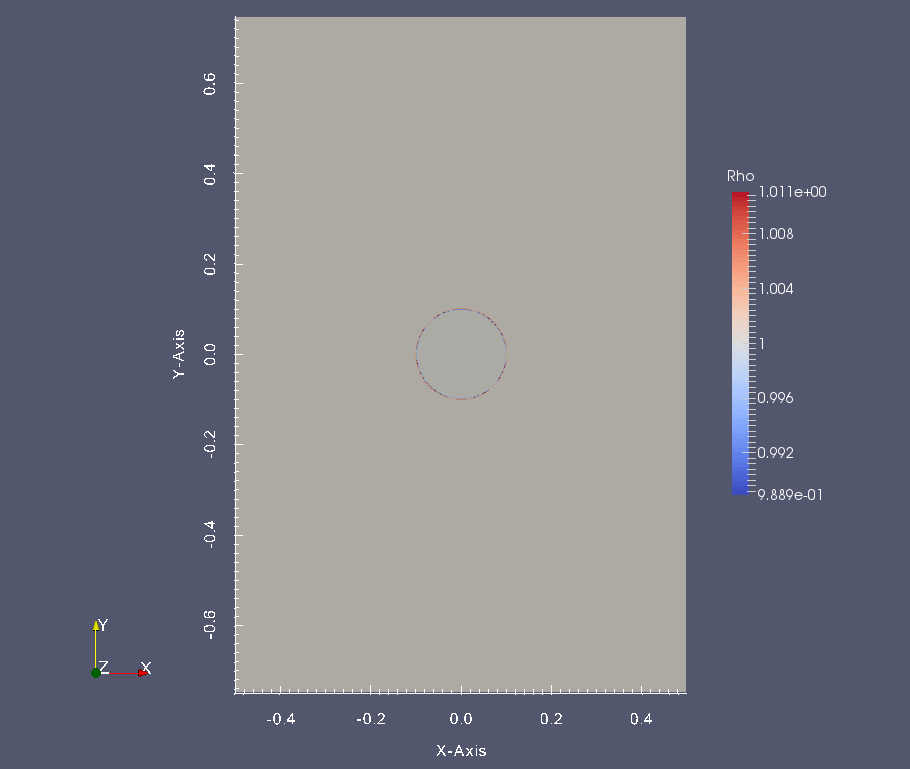
\includegraphics[width=0.4\textwidth]{img/0-density.png}
    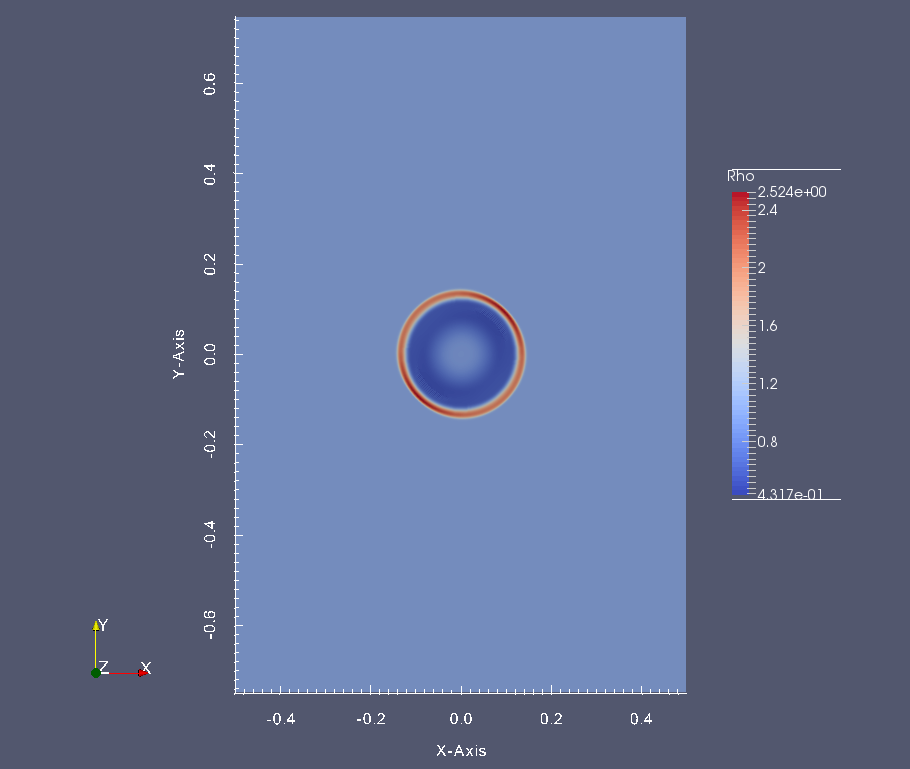
\includegraphics[width=0.4\textwidth]{img/5-density.png}
\end{center} 
\caption{Plasma density in $t = 0$ and $t = 0.03s$.}
\end{figure} 
\begin{figure}[H]
    \begin{center}
        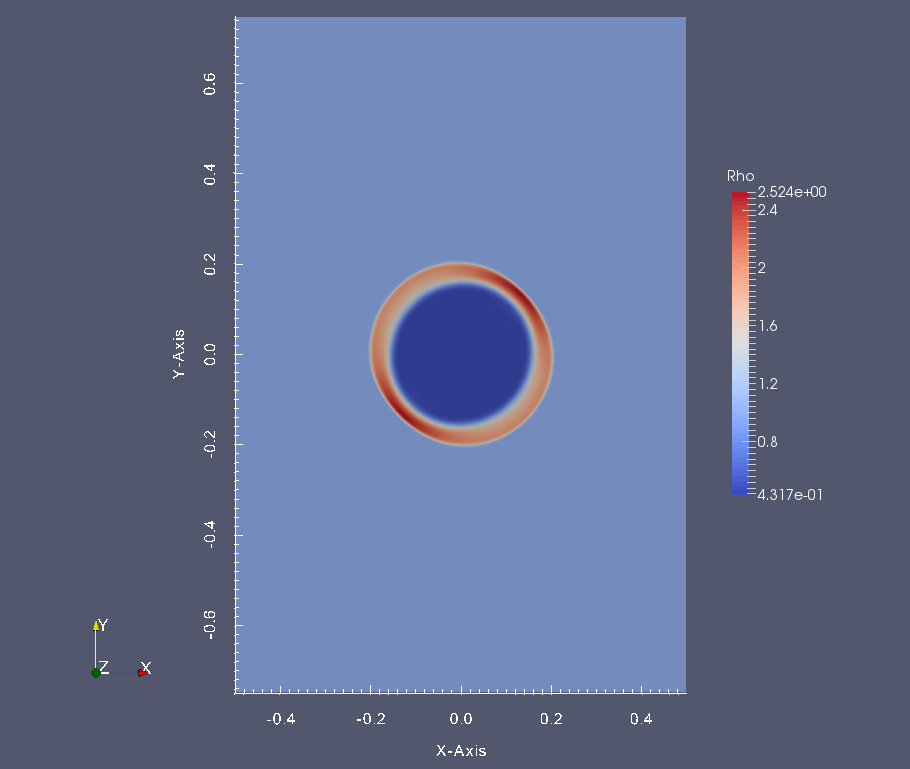
\includegraphics[width=0.4\textwidth]{img/10-density.png}
        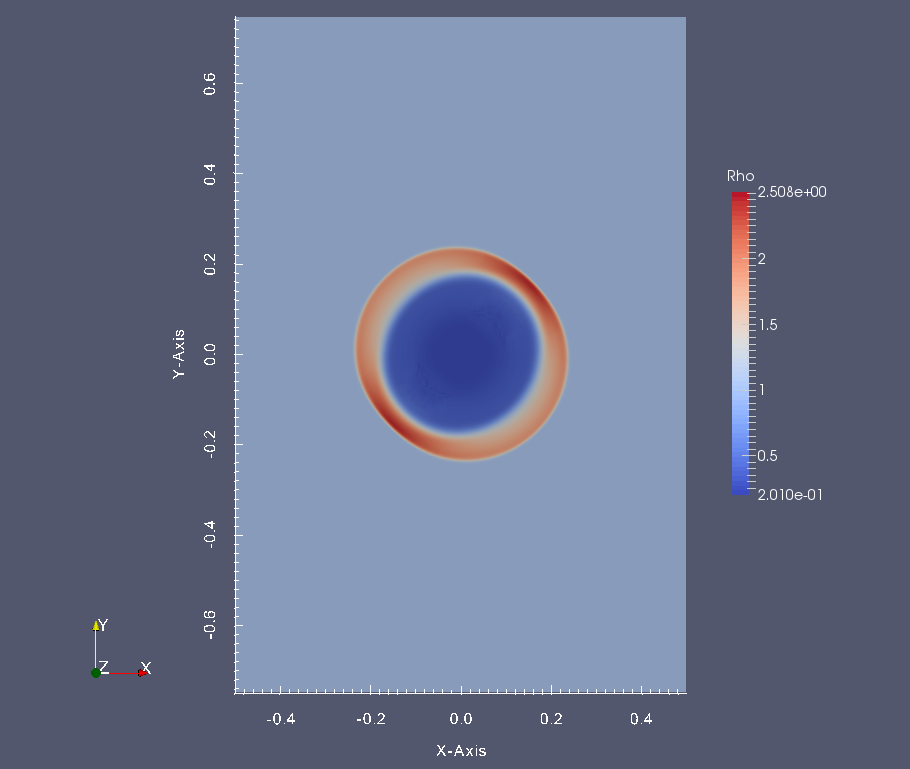
\includegraphics[width=0.4\textwidth]{img/13-density.png}
    \end{center} 
    \caption{Plasma density in $t = 0.12s$ and $t = 0.16s$.}
\end{figure} 
\begin{figure}[H]
    \begin{center}
        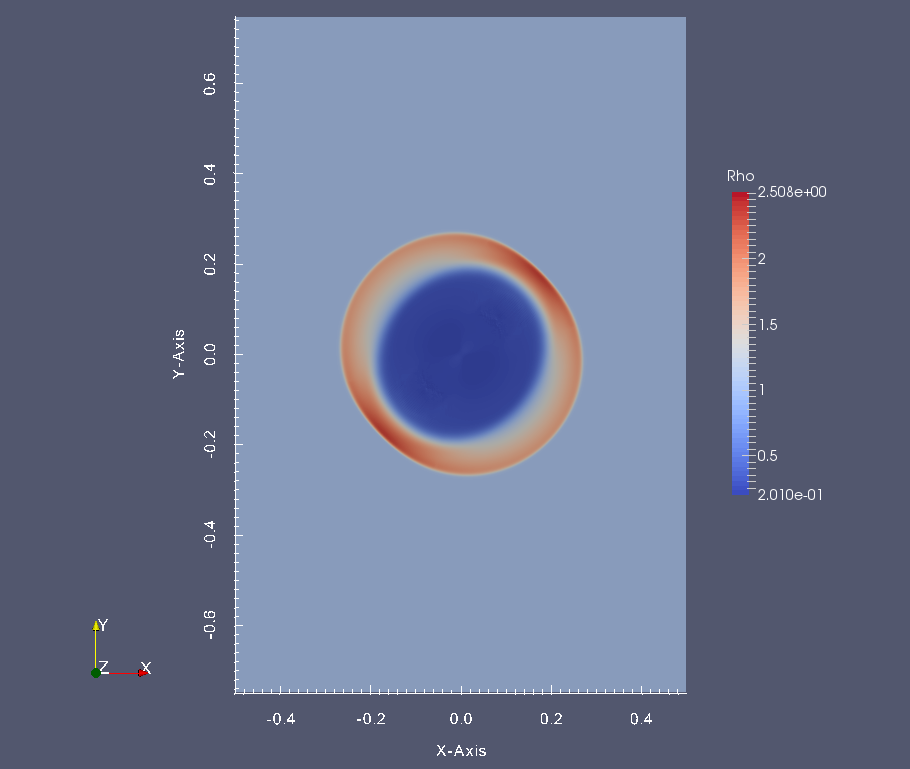
\includegraphics[width=0.4\textwidth]{img/16-density.png}
        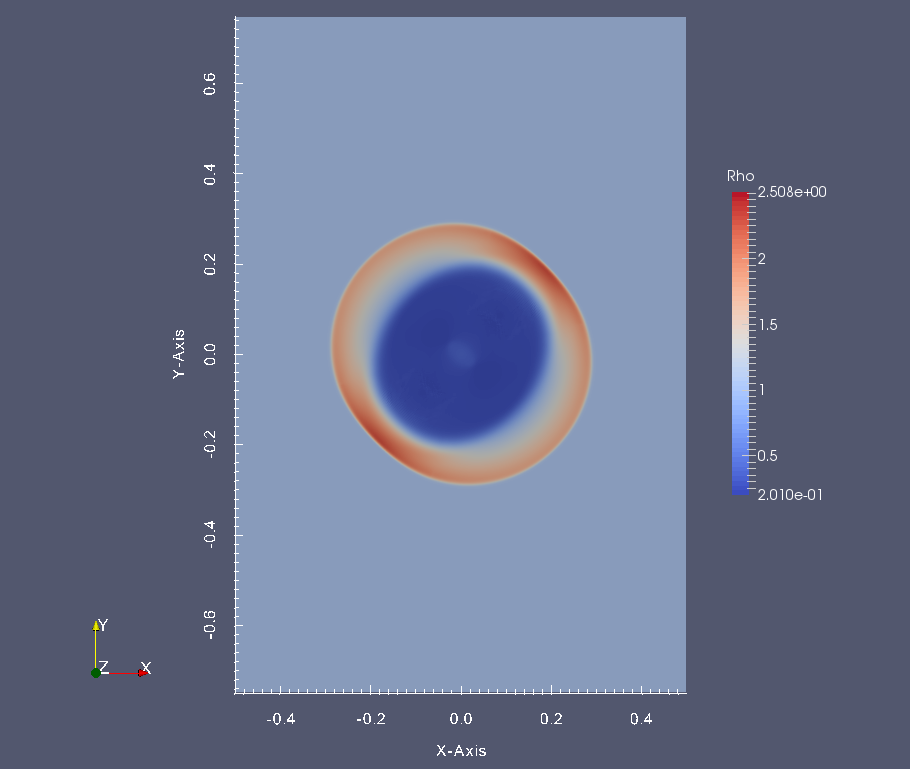
\includegraphics[width=0.4\textwidth]{img/18-density.png}
    \end{center} 
    \caption{Plasma density in $t = 0.19s$ and $t = 0.21s$.}
\end{figure} 
\begin{figure}[H]
    \begin{center}
        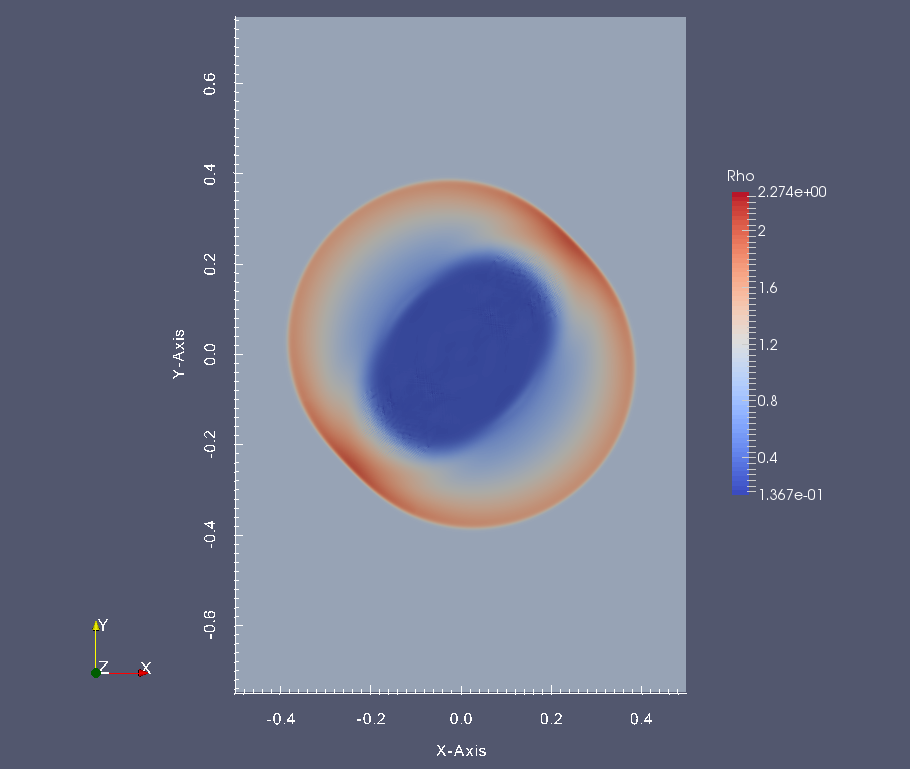
\includegraphics[width=0.4\textwidth]{img/20-density.png}
        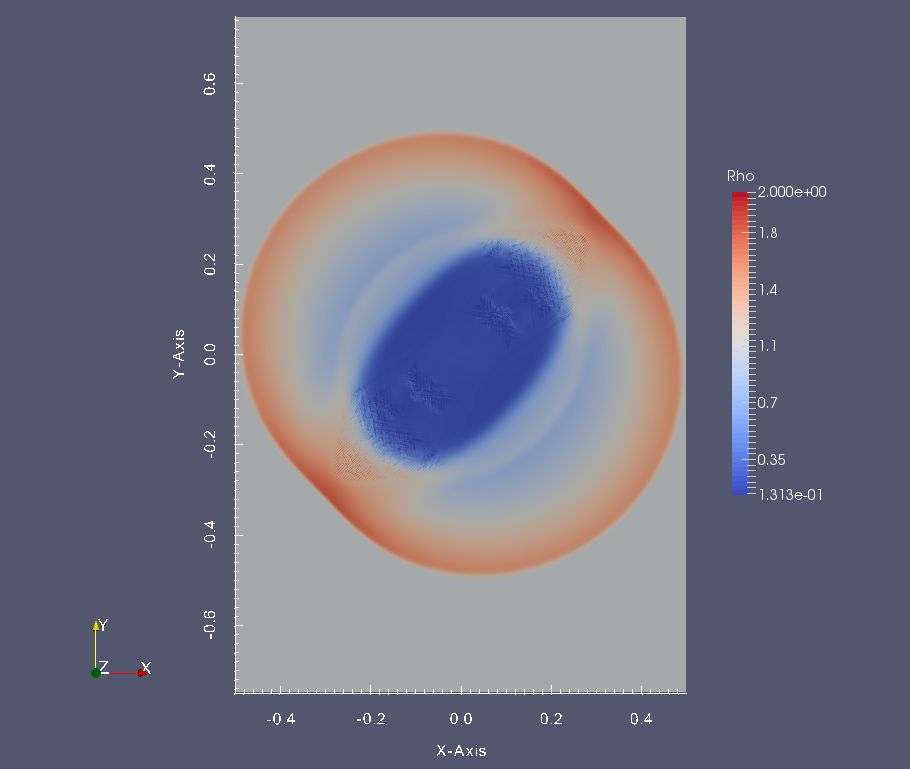
\includegraphics[width=0.4\textwidth]{img/21-density.png}
    \end{center} 
    \caption{Plasma density in $t = 0.32s$ and $t = 0.37s$.}
\end{figure} 

\subsection{Conclusions}
Results are satisfactory in terms of both qualitative and quantitative evaluation. Some non-physical instabilities are present - which will be subject to further study. Generally, results show good agreement with the expected results. The implementation has been proven to be working in an efficient manner, but challenges of real world large-scale problems lie ahead. There is still room for performance improvement, and for implementation of improved algorithms alike, especially with focus on stabilization of the implemented algorithm.

\chapter{Use cases of the implementation}
This chapter will contain one or more real world use cases of the implemented MHD solver in simulating interesting astrophysics problems.

\chapter*{Conclusion, outlook}
Further work will focus on real-world industrial and astrophysical problems, mainly study of the magnetic field reconnection - \cite{reconnection}, and other phenomena occurring both in solar physics and in industrial applications of plasma flow.

\begin{thebibliography}{99}
\addcontentsline{toc}{chapter}{Bibliography}
 \bibitem{1993}Feistauer M.: {\em Mathematical methods in fluid dynamics}, Longman Scientific \& Technical, 1993.

 \bibitem{compress}Feistauer M., Felcman J., Stra�kraba I.: {\em Mathematical and Computational Methods for Compressible Flow}, Oxford University Press, 2003.

 \bibitem{BB}Girault V., Raviart P. - A.:\emph{Finite Element Methods for Navier-Stokes Equations}, Springer, Berlin, 1986.

 \bibitem{SUPG}Lube G.:\emph{Stabilized Galerkin finite element methods for convection dominated and incompressible flow problems}, Num. Anal. and Math. Model. {\bf 29}, Banach Center publications, Warszawa, 1994.

 \bibitem{ALE}Nomura T., Hughes T.J.R.: {\em An arbitrary Lagrangian-Eulerian finite element method for interaction of fluid and a rigid body}, Comp. Methods Appl. Mech. Engrg. {\bf 95} (1992) 115--138.

 \bibitem{Apps_to_aeroel}Sv��ek P., Feistauer M.: \emph{Application of a stabilized FEM to problems of aeroelasticity}, Enumath 2003, Springer, Berlin (2004) 796--805.

 \bibitem{Num_simul_vibr}Sv��ek P., Feistauer M., Hor��ek J.: {\em Numerical simulation of flow induced airfoil vibrations with large amplitudes}, Journal of Fluids and Structures {\bf 23} (2007) 391--411.

\end{thebibliography}

		
\end{document}
